\section{Problemi computazionali nella teoria dei giochi coalizionali}
\subsection{Limitazioni dell'approccio Naive}

Quando utilizziamo una funzione caratteristica per rappresentare un gioco
coalizionale, il problema di trovare una soluzione approccia un
\textbf{utilizzo di memoria pari a} $\mathcal{O}(2^N)$.

\begin{lstlisting}[language=python]
    v = {
        frozenset(['A']): 0,
        frozenset(['B']): 0,
        frozenset(['C']): 0,
        frozenset(['A', 'B']): 1,
        frozenset(['A', 'C']): 1,
        frozenset(['B', 'C']): 1,
        frozenset(['A', 'B', 'C']): 2
    }
\end{lstlisting}

Per quanto riguarda la \textbf{complessità computazionale}, siamo comunque su
$\mathcal{O}(2^N)$.

\begin{lstlisting}[language=python, caption={Controllo che un outcome sia stabile}]
    def is_stable(outcome, cs):
        return all(
            [
                sum([outcome[player] for player in coalition]) >=
                    cs[coalition]
                for coalition in cs
            ]
        )
\end{lstlisting}

\begin{lstlisting}[language=python, caption={Shapley value}]
    def shapley_value(player, cs):
        player = set([player])
        N = len(max(cs, key=len))
        shapley_val = 0

        for coalition in cs:
            s = len(coalition)ma
            marginal_contribution = cs[coalition] - \ cs[coalition - player]

            if marginal_contributoin:
                shapley_val += ((factorial(N-S) * factorial(S-1)) / \ factorial(N)) * marginal_contribution
        return round(shapley_val, 10)
\end{lstlisting}

\begin{quote}
    In che modo possiamo fare meglio?
\end{quote}

\subsection{Strategie per i problemi di computazione}

La soluzione è quella di \textit{concentrarsi} su una categoria specifica di
goichi, che possono essere risolti \textbf{con poco utilizzo di memoria e con
    algoritmi che lavorano in tempo polinomiale}-

Un'altra soluzione è quella di usare alcuni \textbf{algoritmi di
    approssimazioe}, come ad esempio è \textbf{l'algoritmo di Montecarlo}. Questo
algoritmo funziona in tempo polinomiale e nella pratica
\textbf{l'approssimazione dell'errore} è molto piccola nella pratica.

Altra soluzione, è quella di utilizzare delle \textbf{rappresentazoini
    compatte} per la funzione caratteristica. Questo tipo di soluzione ha un
impatto minimo sul consumo della memoria, ha una \textbf{grande espressività},
ovvero che può rappresentare la maggior parte dei giochi e sopratutto
\textbf{lavora in tempo polinomiale.}

\subsection{Gioco del'aereoporto | Airport Game}

\begin{definition}[Airport game]
    Ci sono \textbf{N} compagnie aeree. Ogni compagnia ha bisogno di una pista di atterraggio di una certa lunghezza per i loro aereo.
    Le compagnie, però, possono \textbf{condividere} una pista, e quindi possono unire le forze per \textbf{costruire un'unica pista} abbastanza grande per tutti, e \textbf{dividere i costi}. Come devono fare per \textbf{dividersi i costi?}
\end{definition}

Nella definizione del problema abbiamo un insieme $N = \{1,2,\dots,n\}$ di
giocatori, ai quali ognuno ha associato un costo $c_i$ tale che $c_1 < c_2 <
    \dots < c_n$. La funzione caratteristica è indicata come:

\[
    \nu(S) = \max_{i \in S} c_i \quad \forall S \subseteq N
\]

Cioè, il \textbf{massimo} costo tra i giocatori che fanno parte della
coalizione.

Lo \textbf{shapley value} per il giocatore $i$ in questo gioco viene dato da:

\[
    \Phi_i = \sum_{j=1}^i \frac{c_j - c_{j-1}}{n - j +1}  \forall i \in N; \quad c_0 = 0
\]

\begin{esempio}[Airport game]
\end{esempio}

Immaginiamo di avere \textbf{4} giocatori, quindi 4 compagnie aeree. I costi
sono:
\[
    [8,11,13,18]
\]

\begin{table}[H]
    \begin{center}
        \begin{tabular}{|c|c|c|c|c|c|}
            \hline
            Giocatore       & Aggiungi 1 & Aggiungi 2 & Aggiungi 3 & Aggiungi 4 & Shapley value \\
            \hline
            Costi marginali & 8          & 3          & 2          & 5          &               \\
            \hline
            Costo P1        & 2          &            &            &            & 2             \\
            \hline
            Costo P2        & 2          & 1          &            &            & 3             \\
            \hline
            Costo P3        & 2          & 1          & 1          &            & 4             \\
            \hline
            Costo P4        & 2          & 1          & 1          & 5          & 9             \\
            \hline
        \end{tabular}
    \end{center}
\end{table}
Il gioco dell'aeroporto, noto anche come Airport Game, coinvolge diversi giocatori che collaborano per contribuire
ai costi associati all'aggiunta di servizi all'aeroporto.
Ciascun giocatore può scegliere di aggiungere una quantità
specifica di servizio, ognuna associata a un costo marginale.
Il valore di Shapley è una misura di quanto ciascun giocatore
dovrebbe contribuire in modo equo ai costi totali, considerando
il loro contributo al gioco. Questo calcolo si basa sulla
cooperazione tra i giocatori e assicura una distribuzione
equa dei costi totali.

\subsection{Approssimazione di Montecarlo}

\begin{definition}[Approssimazione di montercarlo]
    L'approssimazione di Montecarlo è un metodo di calcolo che si basa su
    \textbf{numeri casuali} per ottenere un risultato approssimato.
\end{definition}

Nel nostro caso, supponiamo di avere una \textit{distribuzione di probabilità}
$P(X)$ e che volessimo calcolarci $P(x)$.

\textbf{Idea 1:} Approssimiamo $P(x)$ usando delle frequenze semplici.

\textbf{Idea 2:} Generiamo un campione $D$ di grandezza $M$ da $P(X)$ e calcoliamo $P(x)$.

\[
    P_D(X=x) = \frac{M_{X=x}}{M}
\]

cioè, calcoliamo la probabilità che $X$ sia uguale a $x$ nel campione $D$.

Confrontiamo ora la \textbf{formula dello Shapley Value} originale:

\[
    \shapleyval
\]

con:
\begin{itemize}
    \item $\pi_N$ l'insieme di tutte le possibili permutazioni di N
    \item $B(\pi, i)$ L'insieme di tutti i predecessori di $i$ nella permutazione $\pi$
\end{itemize}

Invece, la formula dello Shapley Value approssimata con la tecnica di
montecarlo è:
\[
    \textcolor{red}{\widetilde{\phi}(i,\nu)} = \frac{1}{\textcolor{red}{m}} \sum_{\textcolor{red}{\pi \in \mathcal{P}}} \nu(B(\pi,i) \cup \{i\}) - \nu(B(\pi,i))
\]

dove:

\begin{itemize}
    \item $\mathcal{P} \subset \prod_N$ è il \textbf{sottoinsieme} di tutte le possibili permutazioni di N
    \item $B(\pi,i)$ è l'insieme di tutti i predecessori di $i$ nella permutazione $\pi$.
\end{itemize}

Un esempio di \textit{pseudo-codice} per l'approssimazione è il seguente:

\begin{esempio}[Pseudo codice Shapley Value con Montecarlo]
\end{esempio}

%mathescape for lstlisting
\begin{lstlisting}[language=Python, mathescape]
    #Input: v $\rightarrow$ characteristic function; m $\rightarrow$ numero di sample
    def MC_Shapley($v,m$):
        $\widetilde{\phi_i} = 0$ $\forall i \in N$
        for k = 1,...,m:
            $\pi_k$ = permutazione casuale di $N$
            for i = i,...,n:
                $sv = v(B(\pi,i)\cup\{i\} - v(B(\pi,i)))$
                $\widetilde{\phi_i} += sv$
        for k = 1,...,n:
            $\widetilde{\phi_i} = \frac{\widetilde{\phi_i}}{m}$
        return $\widetilde{\phi_1}, \widetilde{\phi_2}, ..., \widetilde{\phi_n}$
\end{lstlisting}

Lo pseudocodice rappresenta un algoritmo per calcolare i valori di Shapley
approssimati mediante il metodo del campionamento Monte Carlo (MC\_Shapley).
L'obiettivo dell'algoritmo è stimare i valori di Shapley per un insieme di
giocatori (N) basandosi su una funzione caratteristica (v) e un numero
specifico di campioni (m).

L'algoritmo utilizza un processo di campionamento Monte Carlo per calcolare una
stima approssimata dei valori di Shapley. Per ogni campione, vengono generate
permutazioni casuali degli insiemi di giocatori $(\pi_k)$ e calcolate le
differenze nei valori caratteristici (sv) quando un giocatore viene aggiunto a
un insieme e poi rimosso. Queste differenze vengono sommate per ogni giocatore,
accumulando una stima approssimata dei loro valori di Shapley
($\widetilde{\phi_i}$).

Dopo aver completato il numero desiderato di campioni, il valore
$\widetilde{\phi_i}$ per ciascun giocatore viene normalizzato dividendo per il
numero di campioni (m). Alla fine, l'algoritmo restituisce le stime
approssimate dei valori di Shapley per ogni giocatore.

Questo approccio è utilizzato per affrontare il calcolo dei valori di Shapley
in situazioni in cui non è possibile calcolarli in modo esatto, ma è possibile
ottenere una stima accurata utilizzando il campionamento Monte Carlo.

\subsection{Rappresentazioni compatte}

Lo scopo delle \textbf{rappresentazioni compatte} è quello di ridurre l'impatto
sulla memoria della funzione caratteristica, usando delle strutture a mo di
\textbf{rete}.

Il valore di una coalizione non sarà più accessibili in $\mathcal{O}(1)$ come
avveniva prima utilizzando il metodo Naive. Quello che si ottiene è un
\textbf{tempo polinomiale}.

Avendo questa rappresentazione compatta, sfruttando la proprietà dello Shapley
Value, ci permette di calcolare lo shapley value \textbf{in tempo polinomiale.}

\begin{definition}[Gioco del grafo indotto (ISG)]
\end{definition}

In questa rappresentazione, i \textbf{giocatori} sono dei nodi nel grafo. Gli
archi sono le \textbf{coalizioni} di due giocatori. I pesi degli archi sono il
\textbf{valore delal coalizione}.

Un gioco dei gioco del grafo indotto può essere espresso mediante questa
funzione caratteristica:

\[
    v(C) = \sum_{i,j \subseteq C} w_{ij}
\]

E possiamo calcolare lo shapley value per il player $i$ nel seguente modo:

\[
    \phi_i = w_{ii} + \frac{1}{2} \sum_{j \in \Gamma(i)} w_{ij}
\]

dove:
\begin{itemize}
    \item $w_{ii}$ è il peso dell'arco tra il nodo $i$ e se stesso
    \item $\Gamma(i)$ è l'insieme dei vicini del nodo $i$
\end{itemize}

\begin{figure}[H]
    \begin{center}
        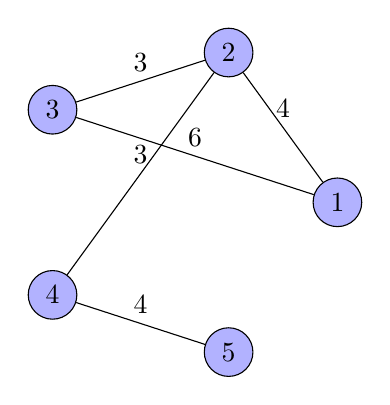
\begin{tikzpicture}
            % Nodi
            \foreach \x in {1,2,3,4,5} {
                    \node[circle, draw, fill=blue!30] (\x) at ({(\x-1)*72}:2) {\x};
                }

            % Archi con pesi
            \draw (1) -- (2) node[midway, above] {4};
            \draw (1) -- (3) node[midway, above] {6};
            \draw (2) -- (3) node[midway, above] {3};
            \draw (2) -- (4) node[midway, above] {3};
            \draw (4) -- (5) node[midway, above] {4};
        \end{tikzpicture}
    \end{center}
    \caption{Esempio di grafo indotto}
\end{figure}

Ora, vediamo un paio di esempio di \textit{coalizioni}.

\begin{esempio}[Coalizioni nel grafo indotto]
\end{esempio}

\begin{figure}[H]
    \begin{center}
        \textbf{Coalizione: $\{1,2,4\}$}

        Il valore $\textbf{v(1,2,4)} = 4 + 3 = 7$

        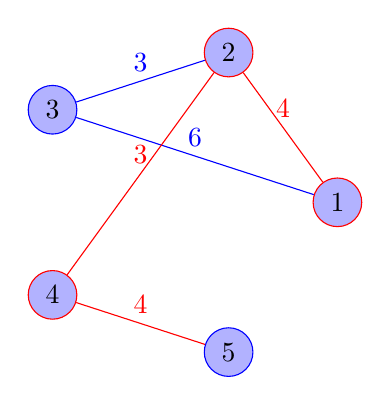
\begin{tikzpicture}
            % Nodi
            \foreach \x/\col in {1/red, 2/red, 3/blue, 4/red, 5/blue} {
                    \node[circle, draw=\col, fill=blue!30] (\x) at ({(\x-1)*72}:2) {\x};
                }

            % Archi con pesi
            \foreach \x/\y/\weight/\col in {1/2/4/red, 1/3/6/blue, 2/3/3/blue, 2/4/3/red, 4/5/4/red} {
                    \draw[\col] (\x) -- (\y) node[midway, above] {\weight};
                }
        \end{tikzpicture}

    \end{center}
    \caption{Esempio coalizione GF (1)}
\end{figure}

\begin{figure}[H]
    \begin{center}
        \textbf{Coalizione: $\{1,2,5\}$}

        Il valore $\textbf{v(1,2,5)} = 4 $

        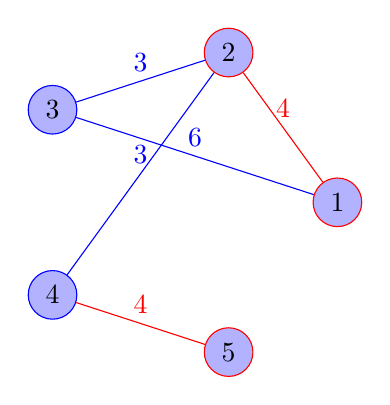
\begin{tikzpicture}
            % Nodi
            \foreach \x/\col in {1/red, 2/red, 3/blue, 4/blue, 5/red} {
                    \node[circle, draw=\col, fill=blue!30] (\x) at ({(\x-1)*72}:2) {\x};
                }

            % Archi con pesi
            \foreach \x/\y/\weight/\col in {1/2/4/red, 1/3/6/blue, 2/3/3/blue, 2/4/3/blue, 4/5/4/red} {
                    \draw[\col] (\x) -- (\y) node[midway, above] {\weight};
                }
        \end{tikzpicture}

    \end{center}
    \caption{Esempio coalizione GF (2)}
\end{figure}

Calcoliamo ora \textbf{lo shapley value}.

Ricordiamo la formula:
\[
    \phi_i = w_{ii} + \frac{1}{2} \sum_{j \in \Gamma(i)} w_{ij}
\]

dove:
\begin{itemize}
    \item $w_{ii}$ è il peso dell'arco tra il nodo $i$ e se stesso
    \item $\Gamma(i)$ è l'insieme dei vicini del nodo $i$
\end{itemize}

Per ogni giocatore $i$, calcoliamo:

\begin{itemize}
    \item $\phi_1 = \frac{1}{2} (4 + 6) = 5$
    \item $\phi_2 = \frac{1}{2} (4 + 3 + 3) = 5$
    \item $\phi_3 = \frac{1}{2} (6 + 3 + 4) = 6.5$
    \item $\phi_4 = \frac{1}{2} (4 + 3 + 4) = 5.5$
    \item $\phi_5 = \frac{1}{2} (4) = 2$
\end{itemize}

\subsection{Reti di contribuzione marginale |MC-Nets}
%metti una label per fare ref
\label{MCnets}

L'idea di questo tipo di reti è quello di rappresentare la \textbf{funzione
    caratteristica} come un'insieme di regole della forma:
\[
    pattern \rightarrow value
\]

Il \textbf{pattern} è una formula booleana su $N$ e il valore associato ad egli
è il suo \textbf{contributo marginale}.

Se un pattern è nella forma $\{a \land b \land \cdots \land c\}$ il valore
associato può essere sia \textit{positivo} che \textit{negativo}, possiamo
\textbf{rappresentare ogni gioco.}

\begin{definition}
    [MC-Nets]
    Una \textbf{rete di contribuzione marginale} è una rete che rappresenta una
    funzione caratteristica $v$ come un insieme di regole della forma:
    \[
        pattern \rightarrow value
    \]

    dove:
    \begin{itemize}
        \item $pattern$ è una formula booleana su $N$
        \item $value$ è il contributo marginale
    \end{itemize}
\end{definition}

\begin{esempio}[MC-Nets]
\end{esempio}

\[
    \begin{aligned}
        \{a \land b\} \rightarrow 5 \\
        \{b\} \rightarrow 2
    \end{aligned}\]

rappresenta la seguente funzione caratteristica:
\[
    \nu(\emptyset) = 0; \nu(\{a\}) = 0; \nu(\{b\}) = 2; \nu(\{a,b\}) = 5 + 2 = 7
\]

Per capire per bene come funziona, diciamo che \textit{dobbiamo sommare i
    valoriper ogni regola che si applica ad una determinata coalizione che si va a
    controllare}.

Una regola $r$ per applicarsi deve essere \textbf{sotto-insieme della
    coalizione} che si sta andando a controllare.

\begin{esempio}[MC-Nets coalizione \{a\}]

\end{esempio}

Se dobbiamo controllare la coalizione $\{a\}$, vediamo quali regole si
applicano.

Ricordiamo il nostro insieme di regole:

\[
    \begin{aligned}
        \{a \land b\} \rightarrow 5 \\
        \{b\} \rightarrow 2
    \end{aligned}
\]

Controlliamo la prima regola: $\{a \land b\} \rightarrow 5$.
\[
    \{a,b\} \nsubseteq \{a\}
\]

In questo caso, la regola \textbf{non si applica} poiché $\{a,b\}$ non è sottoinsieme di
$\{a\}$. 

Controlliamo la seconda regola: $\{b\} \rightarrow 2$.

\[
    \{b\} \nsubseteq \{a\}    
\]

Anche in questo caso, la regola \textbf{non viene applicata.}P

Allora, siccome dobbiamo sommare il valore di ogni regola che viene applicata, per la coalizione $\{a\}$ la somma è:
\[
    0+0 = 0    
\]

Quindi, assegniamo alla coalizione $\{a\}$ il valore $0$.

\begin{esempio}[MC-Nets coalizione \{a,b\}]
\end{esempio}

Se dobbiamo controllare la coalizione $\{b\}$, vediamo quali regole si
applicano.

Anche qui, le regole sono le stesse:
\[
    \begin{aligned}
        \{a \land b\} \rightarrow 5 \\
        \{b\} \rightarrow 2
    \end{aligned}
\]

Controlliamo la prima regola: $\{a \land b\} \rightarrow 5$.

\[
    \{a,b\} \nsubseteq \{b\}
\]

In questo caso, la regola \textbf{non si applica} poiché $\{a,b\}$ non è sottoinsieme di
$\{b\}$.

Controlliamo la seconda regola: $\{b\} \rightarrow 2$.

\[
    \{b\} \subseteq \{b\}
\]

In questo caso, la regola \textbf{si applica} poiché $\{b\}$ è sottoinsieme di
$\{b\}$. Segniamo quindi il valore della regola, ovvero $2$.

Allora, siccome dobbiamo sommare il valore di ogni regola che viene applicata, per la coalizione $\{b\}$ la somma è:
\[
    2 + 0 = 2
\]

Quindi, assegniamo alla coalizione $\{b\}$ il valore $2$.

\begin{esempio}[MC-Nets coalizione \{a,b\}]

\end{esempio}

Dobbiamo controllare l'ultimo caso. Se dobbiamo controllare la coalizione $\{a,b\}$, vediamo quali regole si
applicano.

Anche qui, le regole sono le stesse:
\[
    \begin{aligned}
        \{a \land b\} \rightarrow 5 \\
        \{b\} \rightarrow 2
    \end{aligned}
\]

Controlliamo la prima regola: $\{a \land b\} \rightarrow 5$.

\[
    \{a,b\} \subseteq \{a,b\}
\]

In questo caso, la regola \textbf{si applica} poiché $\{a,b\}$ è sottoinsieme di
$\{a,b\}$. Segniamo quindi il valore della regola, ovvero $5$.

Controlliamo la seconda regola: $\{b\} \rightarrow 2$.

\[
    \{b\} \subseteq \{a,b\}
\]

Anche in questo caso, la regola \textbf{si applica} poiché $\{b\}$ è sottoinsieme di
$\{a,b\}$. Segniamo quindi il valore della regola, ovvero $2$.

Allora, siccome dobbiamo sommare il valore di ogni regola che viene applicata, per la coalizione $\{a,b\}$ la somma è:

\[
    5 + 2 = 7
\]

Quindi, assegniamo alla coalizione $\{a,b\}$ il valore $7$.

Abbiamo ottenuto quindi tutti i valori che ci servono per calcolare lo shapley value.

\begin{itemize}
    \item \{a\} $\rightarrow$ 0
    \item \{b\} $\rightarrow$ 2
    \item \{a,b\} $\rightarrow$ 7
\end{itemize}

Lo \textbf{shapley value} nel caso delle $MC-Nets$ è dato da:
\[
    \phi_i = \sum_{\varphi \rightarrow x \in rs_i} \frac{x}{|\varphi|}     
\]

dove:
\begin{itemize}
    \item $x$ è il valore della regola $\varphi \rightarrow x$
    \item $|\varphi|$ è la cardinalità della regola
    \item $rs_i$ è l'insieme di tutte le regole che si applicano al giocatore $i$
\end{itemize}

Dobbiamo, quind, prendere solo le regole che si applicano al giocatore $i$.

Iniziamo con il giocatore \textbf{\{a}\}.

L'unica regola che si applica è quella di $\{a,b\} \rightarrow 5$.

Quindi, il calcolo è:

\[
    \phi_a = \frac{5}{2} = 2.5  + 0
\]

Passiamo al giocatore \textbf{\{b}\}.

Si applicano 2 regole: $\{b\} \rightarrow 2$ e $\{a,b\} \rightarrow 5$.

Quindi, il calcolo è:

\[
    \phi_b = \frac{2}{1} + \frac{5}{2} = 4.5
\]

Abbiamo quindi calcolato \textbf{lo shapley value} per ogni giocatore.